\documentclass{article}

\usepackage{graphicx}
\usepackage{multirow}

\title{Note: Linear Regression with Multiple Variables}
\author{Sun Zhao}

\begin{document}
\maketitle
\newpage

\section{Multiple Features}
Univariate linear regression takes only one variable to predict values. Mostly, values are relevant to multiple features other than one feature. Multiple features are powerful than single
 feature to predict values. An example of multiple features are shown in Table\ref{multivate_feature_example}. A house's price is now related to the size, number of bedrooms, number of floors, and age of it. Each row is an training example with left three feature columns and right one value column. We use n to denote the number of features, $x^{(i)}$ to denote the features of the $i^{th}$ training example and $x^{(i)}_{j}$ to denote the value of feature j in $i^{th}$ training example. For example, $x^{(2)}$ equals $[1416 \quad 3 \quad 2 \quad 40]^{T}$ and $x^{(2)}_{3}$ equals 2. Since the hypothesis of univariate linear regression is $h_{\theta}(x) = \theta_{0} + \theta_{1}x$, that of multivariate linear regression becomes formula\ref{hypothesis}.
 
\begin{table}[ht]
\begin{center}
\caption{}\label{multivate_feature_example}
\begin{tabular}{c|c|c|c|c}
\hline
size($feet^{2}$) & \# of bedrooms & \# of floors & Age(years) & Price(\$1000)\\
\hline
2014    &   5   &   1   &   45  &   460\\
1416    &   3   &   2   &   40  &   232\\
1534    &   3   &   2   &   30  &   315\\
852     &   2   &   1   &   36  &   178\\
\ldots & \ldots &  \ldots & \ldots & \ldots\\
\end{tabular}
\end{center}
\end{table}

\begin{equation}\label{hypothesis}
   h_{\theta}(x) = \theta_{0} + \theta_{1}x_{1} + \theta_{2}x_{2} + \ldots + \theta_{n}x_{n}
\end{equation}
Let $x^{(i)}_{0}$ = 1, $\theta = [\theta_{0} \quad \theta_{1} \ldots \theta_{n}]^{T}$, and $x = [x_{0} \quad x_{1} \quad \ldots x_{n}]^{T}$, then formula1 is refined as formula\ref{hypothesis_refine}.

\begin{equation}\label{hypothesis_refine}
 h_{\theta}(x) = {\theta}^{T}x
\end{equation}

\section{Gradient Descent}
Refer to formula1 we can infer the cost function of multivariate linear regression shown in formula\ref{cost_function}.
\begin{equation}\label{cost_function}
  J(\theta_{0}, \theta_{1}, \ldots , \theta_{n}) = \frac{1}{2m} \sum_{i=1}^{m} (h_\Theta({x^{(i)}})-y^{(i)})^2
\end{equation}
And the gradient descent algorithm is adapted to:
\medskip
\hrule
\smallskip
Algorithm1: Gradient for Multivariate Linear Regression
\smallskip
\hrule
\smallskip
Repeat\{\\
$\theta_j=\theta_j - \alpha \frac{1}{m} \sum_{i=1}^{m}(h_\theta(x^{(i)})-y^{(i)}) \cdot x^{(i)}_{j}$\\
\}\\
\hrule

\section{Practical Issues}
\subsection{Feature Scaling}
The idea of feature scaling is to make sure that all features are on similar scale. If one feature's range is significantly dominating the others', the regression process will converge at a very slow speed. Generally, make the scale of all features is around [-1, 1] is a good choice. Methods for normalization includes dividing values by its ranges or first decreasing by its mean values and then dividing by its range. In a word, we can normalize x form [min, max] with x/(max-min) or (x-average([min, max]))/(max-min).
\subsection{Learning Rate}
The core function of gradient descent is $\theta_j =\theta_j - \alpha\frac{\partial}{\partial \theta_j}J(\theta)$. When running gradient descent algorithm, we need to choose an appropriate $\alpha$ and make sure the algorithm is working correctly. Teacher recommended to plot the value of $J(\theta)$ against the number of regression iterations. If the plotted curve decreases faster as Figure1(A), then we can confirm $\alpha$ and the algorithm all works well. If the plotted curve decreases slow as Figure\ref{learning_rate_choice}(B), we need to increase the value of $\alpha$ a little more. Otherwise, the plotted curve increase as Figure\ref{learning_rate_choice}(C) or vibrates as Figure\ref{learning_rate_choice}(D), we have to decrease the value of $\alpha$.

\begin{figure}[ht]
  \centering
  % Requires \usepackage{graphicx}
  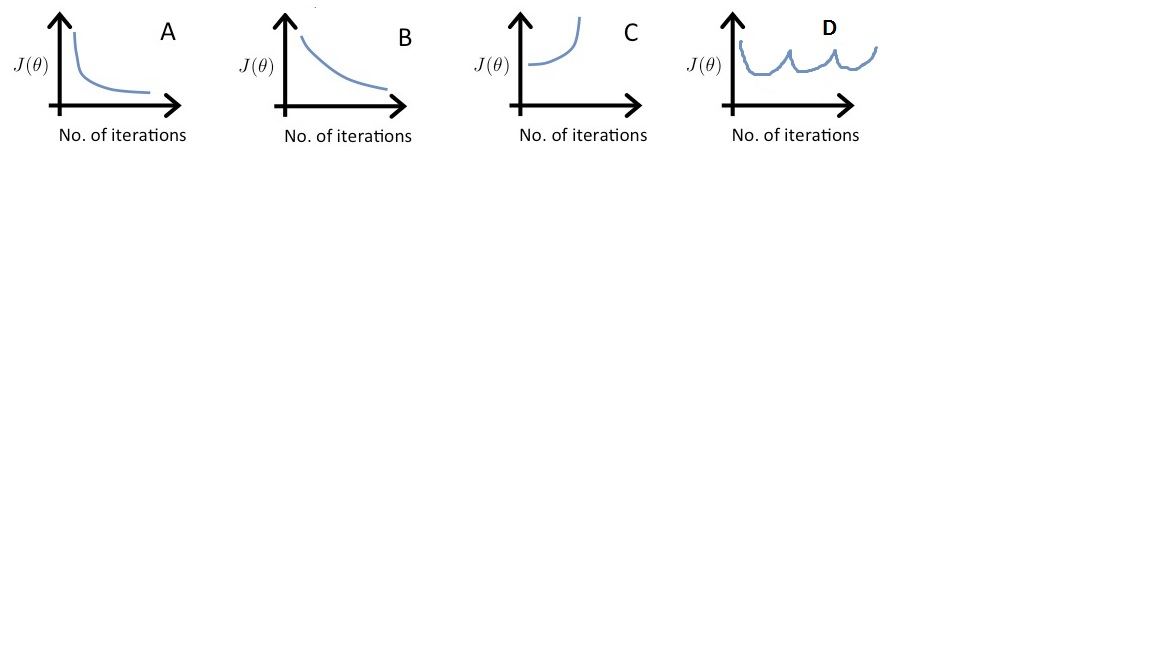
\includegraphics[width=10cm]{Figure1.jpg}\\
  \caption{}\label{learning_rate_choice}
\end{figure}

\subsection{Choosing Features}
Generally, we can adopt three rules to choose features:
\begin{itemize}
\item Feature generalization.
\item Feature reduction.
\item Polynomial feature
\end{itemize}
Feature generalization suggests that generalized feature is often better than multiple combined features. For example, when predicting the price of a house, the area is a good generalized feature than combined features with frontage and depth. When talking about feature reduction, we mean that features relevant to others should be removed and treated as redundant features. Since values may not be linearly relevant to features, we can use polynomial features such as square features, cubic features et. As polynomial feature is adopted, the hypothesis function may be like $h_{\theta}(x) = \theta_{0} + \theta_{1}x_{1} + \theta_{2}x_{2}^{2} + \theta_{3}x_{3}^{3}$. Let $y_{1} = x_{1}, y_{2} = x_{2}^{2}, y_{3} = x_{3} ^ {3}$, the hypothesis is reduced to $h_{\theta}(y) = \theta_{0} + \theta_{1}y_{1} + \theta_{2}y_{2} + \theta_{3}y_{3}$ which is a linear regression hypothesis.
\section{Normal Equation}
Gradient descent solves linear regression literately, however, normal equation solves it in a analytical way. Recall that the cost function of linear regression is $J(\theta) = \frac{1}{2m} \sum_{i=1}^{m} (h_\Theta({x^{(i)}})-y^{(i)})^2$ and according to normal equation, let $\frac{\partial}{\partial \theta_j}J(\theta_j, \theta_1) = 0$ (for j = 0 \ldots m), and we will get a system of equations. Applying $J(\theta) = \frac{1}{2m} \sum_{i=1}^{m} (h_\Theta({x^{(i)}})-y^{(i)})^2$, the linear algebra form of normal equation is:
\begin{equation}\label{normal_quation_linear_algebra form}
X^{T}X\theta - X^{T}Y = 0
\end{equation}
thus,
\begin{equation}\label{theta_expression}
\theta = (X^{T}X)^{-1}X^{T}Y
\end{equation}
The advantages and disadvantages comparison between gradient descent and normal equation is shown in Table\ref{normal_equation_comparison_with_gradient_descent}.
\begin{table}[ht]
\begin{center}
\caption{}\label{normal_equation_comparison_with_gradient_descent}
\begin{tabular}{l|l}
\hline
Gradient Descent & Normal Equation\\
\hline
Need to choose $\alpha$ & No need to choose $\alpha$\\
Need many iterations & No iterations\\
Works well when n is large & Slow if n is large\\
No need to compute matrix & Need to compute $(X^{T}X)^{-1}$\\
\hline
\end{tabular}
\end{center}
\end{table}
\section{Summary}
Multivariate linear regression takes advantage of multiple features and is much powerful than univariate linear regression. When using gradient descent algorithms, we should take care of choosing appropriate features and learning rate. If the number of examples is not very large, normal equation is a faster alternative.
\end{document}
